
\documentclass{article} % For LaTeX2e
\usepackage[submission]{colm2026_conference}

\usepackage{microtype}
\usepackage{hyperref}
\usepackage{url}
\usepackage{booktabs}
\usepackage{multirow}
\usepackage{xcolor}
\usepackage{graphicx}

% NOTE: including geometry package
% The geometery package modifies some page properties when used. This can dramatically change the page margins, aleading to severe template violation, and potential desk rejection. If the package is required, it can be used with the "pass" flag to skip the default page modifications, as in the following line:
% \usepackage[pass]{geometry}

\usepackage{lineno}

\definecolor{darkblue}{rgb}{0, 0, 0.5}
\hypersetup{colorlinks=true, citecolor=darkblue, linkcolor=darkblue, urlcolor=darkblue}


\title{Curing Context Pollution: Externalized Executive Function\\for Multi-Turn LLM Conversations}

% Authors must not appear in the submitted version.
\author{Anonymous Authors}

\newcommand{\fix}{\marginpar{FIX}}
\newcommand{\new}{\marginpar{NEW}}

\begin{document}

\ifcolmsubmission
\linenumbers
\fi

\maketitle

\begin{abstract}
Large language models degrade in extended multi-turn conversations as the assistant's own prior outputs accumulate and act as context pollution, anchoring future generation on earlier (potentially incorrect) reasoning. The model over-conditions on its own responses and struggles to update its approach when the user provides new or correcting information. We frame this as a deficit of \emph{executive function}: the higher-order cognitive capacity for monitoring one's own reasoning, flexibly updating beliefs when they conflict with new evidence, and inhibiting responses anchored on unproductive approaches. We propose \emph{context editing as externalized executive function}, in which a separate self-review agent identifies where the assistant's approach has been invalidated by the user's requirements, where errors have been carried forward, or where unproductive reasoning has accumulated, then rewrites the context to preserve correct work while removing what is harmful. Across math, code, database, function-calling, real human--AI conversations, and agentic tool-use settings, our approach substantially improves multi-turn performance (e.g., 60\%$\to$90\% on math), with gains that generalize across model families at different scales. We further show that context editing is a learnable skill: a minimal memory-based system accumulates analysis principles from experience and transfers them to unseen conversations without parameter updates. Prior mitigations that simply discard all assistant messages suffice in simple settings but catastrophically fail in agentic settings where state must be tracked (55\%$\to$0\%), demonstrating that selective context editing is necessary for complex multi-turn interactions.
\end{abstract}


%% ============================================================
\section{Introduction}
\label{sec:intro}
%% ============================================================

Multi-turn conversation is the dominant mode of interaction with large language models, especially as agentic AI systems place models in long, stateful dialogues with humans and tools. Yet LLMs perform substantially worse in multi-turn settings than on equivalent single-turn tasks. \citet{laban2025lost} showed that accuracy drops 39\% on average across 15 models and 6 task domains---even across conversations spanning only a handful of turns. \citet{huang2026context} identified the primary cause: \emph{context pollution}, the accumulation of incorrect assumptions, failed approaches, and speculative reasoning in the assistant's own prior messages. This degradation does not require extreme context length; the assistant's own generated tokens act as pollution, anchoring future generation on flawed foundations even when the user explicitly corrects course (Figure~\ref{fig:problem}).

This degradation is not a capability deficit---the model can solve the same problem from scratch. It is a \emph{self-regulation} deficit. In cognitive science, \textbf{executive function} refers to the higher-order processes that manage attention, suppress inappropriate responses, and update working representations when circumstances change~\citep{miyake2000unity,diamond2013executive}. We draw on this framework to characterize the specific failure here: not a single-turn reasoning deficit, but the inability to \emph{self-correct across turns}. A human problem-solver recognizes when an approach is failing, suppresses the impulse to continue, and redirects effort. Current LLMs struggle with this: they cannot selectively ignore their own prior reasoning, even when it has since become invalidated.

Existing mitigations simply discard all assistant messages~\citep{huang2026context,khalid2025ergo}, effectively restarting from scratch each turn. This works when the model can re-derive the answer from user messages alone. But in realistic settings---multi-step coding, iterative design, tool-use agents---the assistant's prior work is essential context. Discarding it is not just wasteful but destructive: on the tau2-bench agentic benchmark~\citep{barres2025tau2}, blanket assistant omission drops performance from 55\% to 0\%.

We propose \emph{context editing via externalized executive function}: a separate self-review agent identifies where the assistant has diverged from the user's intent, where errors have been carried forward, and where unproductive reasoning has accumulated, then rewrites the context to preserve correct work while removing what is harmful (Figure~\ref{fig:method}).

There is a useful irony in this framing. The transformer architecture~\citep{Vaswani+2017} is built around the attention mechanism, which computes relevance weights over all tokens in context. Yet this token-level attention demonstrably fails at the \emph{cognitive} task of selective attention: deciding which prior reasoning to rely on and which to suppress. Our approach uses autoregressive generation---additional LLM calls at test time---to make these harder, deliberate decisions about what deserves attention, compensating for a deficit that the architectural attention mechanism cannot resolve on its own. In this way, our work extends test-time scaling~\citep{wei2022chain,wang2023selfconsistency,yao2024tree} from single-turn settings (scaling compute within one generation) to multi-turn settings (editing the accumulated context presented to the model).

Interestingly, we find that prior assistant messages act as a \emph{cognitive hazard}: even a model prompted as an independent reviewer produces degraded analysis when exposed to them, collapsing performance to baseline or worse (Section~\ref{sec:cognitive-hazard}). Context pollution impairs not just the conversational assistant where we might expect the model to bias towards consistency with its prior messages but \emph{any model processing the same context}, requiring either structural exclusion or other means for addressing the issue.

\paragraph{Contributions.}
\begin{itemize}
    \item We frame multi-turn LLM degradation as a deficit of executive function, providing a unified cognitive-science lens for failure modes previously described in isolation.
    \item We propose context editing via externalized executive function, a self-review agent that selectively edits conversation context to remove pollution while preserving correct work.
    \item We identify that prior assistant messages constitute a \emph{cognitive hazard} that degrades even independent reviewer models, requiring structural exclusion by design.
    \item We evaluate across controlled multi-turn benchmarks (math, code, database, function calling), real human--AI conversations (WildChat), and agentic tool-use tasks (tau2-bench), demonstrating consistent improvement across four model families and showing that our approach succeeds where blanket omission catastrophically fails.
    \item We show that context editing is a learnable skill: without any parameter updates, a memory-based learning system accumulates analysis principles from a small training set and transfers them to unseen conversations, improving win rates by up to +13.8pp on WildChat.
\end{itemize}


\begin{figure}[t]
\centering
% \fbox{\parbox{0.95\linewidth}{\centering\textbf{[Figure 1: Problem illustration.]} A multi-turn conversation where the assistant commits to an incorrect interpretation early on. Later user messages correct the misunderstanding, but the assistant's prior reasoning remains in context and anchors subsequent responses, leading to repeated errors.}}
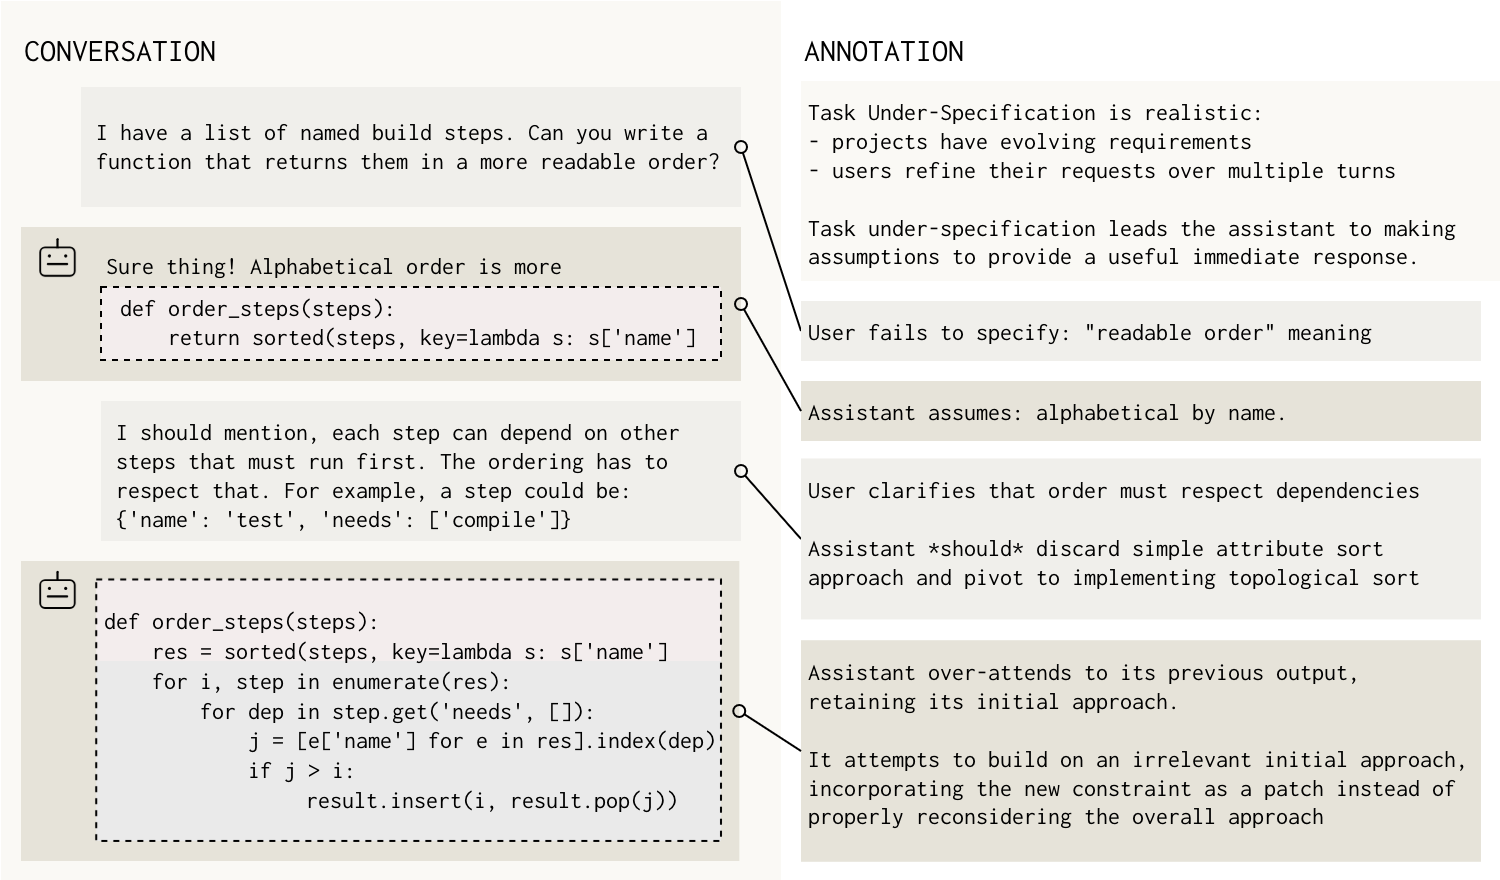
\includegraphics[width=\textwidth]{assets/ctxe_fig1(2).png}
\caption{Context pollution in multi-turn conversations. The assistant's early (incorrect) reasoning persists in context and biases all subsequent generation, even after the user provides correcting information.}
\label{fig:problem}
\end{figure}

\begin{figure}[t]
\centering
% \fbox{\parbox{0.95\linewidth}{\centering\textbf{[Figure 2: Method overview.]} The analyzer reads the conversation in two steps: (1)~extract a clean task specification from user messages only (selective attention), (2)~compare it against the full conversation to identify correct and incorrect assistant work (error monitoring). The result is used to rewrite the context, preserving correct work and removing pollution, before the assistant generates its next response.}}
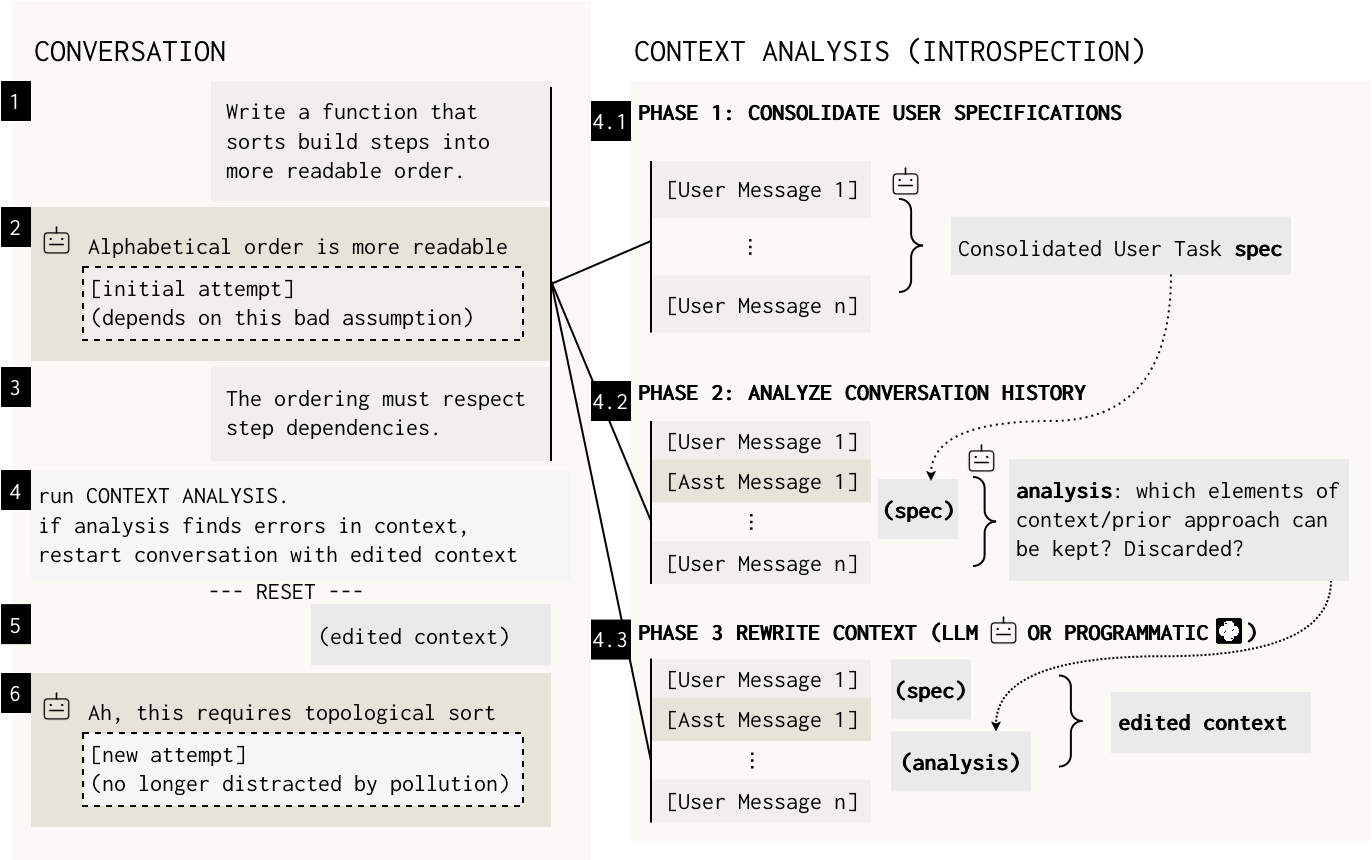
\includegraphics[width=\textwidth]{assets/ctxe_fig2(4).png}
\caption{Context editing via externalized executive function. A separate analyzer agent externalizes the executive functions that LLMs lack: selective attention (filtering out assistant messages during intent extraction) and error monitoring (comparing clean intent against the assistant's actual work).}
\label{fig:method}
\end{figure}

%% ============================================================
\section{Related Work}
\label{sec:related}
%% ============================================================

\paragraph{Multi-turn degradation and context pollution.}
\citet{laban2025lost} introduced the Lost in Conversation (LiC) framework, showing that multi-turn performance drops 39\% on average across 15 LLMs---driven by increased unreliability (+112\%) rather than reduced capability ($-$16\%). \citet{huang2026context} termed this \emph{context pollution} and showed that simply omitting all assistant messages (assistant omission, AO) recovers much of the lost performance across multiple settings, establishing that the assistant's own outputs---not user messages or task difficulty---are the primary source of degradation. \citet{khalid2025ergo} proposed ERGO, which monitors token-level entropy and triggers context resets. Both approaches discard all assistant messages, which is effective only when the model can re-derive answers from scratch. We build on their finding while showing that omission fails catastrophically in agentic settings.

\paragraph{Executive function in cognitive science.}
Executive function refers to the cognitive processes that regulate attention, suppress inappropriate responses, and update working representations~\citep{miyake2000unity}. \citet{diamond2013executive} identifies three core components: inhibitory control, working memory updating, and cognitive flexibility. We use this framework to characterize what LLMs lack in multi-turn settings. The connection is functional, not mechanistic: the \emph{behavioral} failures align with executive function deficits, though we do not claim LLMs share human cognitive architecture. This parallels how \citet{yao2024tree} drew on dual-process theory~\citep{kahneman2011thinking} to motivate tree-structured search for single-turn problems.

\paragraph{Test-time scaling.}
Methods such as chain-of-thought~\citep{wei2022chain}, self-consistency~\citep{wang2023selfconsistency}, and structured search~\citep{yao2024tree} scale inference compute within a single generation. Our work extends test-time scaling to the multi-turn setting: rather than searching over possible outputs, we edit the \emph{input context} presented to the model across turns, investing additional LLM calls to improve the quality of information the model reasons over.

\paragraph{Memory-based self-improvement.}
A growing line of work uses persistent memory to improve LLM capabilities without parameter updates. General-purpose memory systems store and retrieve knowledge for personalization and continuity~\citep{xu2025amem,wang2025mem1}. Agentic memory systems go further, accumulating procedural knowledge and task-specific heuristics that improve agent performance over time: the Dynamic Cheatsheet~\citep{suzgun2025cheatsheet} maintains a mutable text document updated across problem instances; Voyager~\citep{wang2023voyager} builds a skill library for open-ended exploration; and several recent systems learn reusable reasoning strategies~\citep{li2025reasoningbank,gao2025arcmemo,gao2025memp,xie2025evolver,zhao2025agenticce}. A separate thread optimizes the memory system itself rather than the downstream task~\citep{zheng2025memevolve,sun2025alma}. We adapt the Dynamic Cheatsheet for context editing, targeting accumulated analysis principles at the analyzer's executive function rather than the task-solving assistant.

\paragraph{Agentic context management.}
A growing body of work uses LLM-driven context manipulation for long-horizon tasks: THREAD~\citep{mei2025thread} spawns sub-agents with summarized results, Recursive Language Models~\citep{zhang2025rlm} treat context as a programmatically manipulated variable, and Context Folding~\citep{sun2025contextfolding} trains agents to branch and collapse sub-trajectories. These methods target \emph{compaction}---fitting more reasoning into bounded context. Our work addresses a different problem: \emph{context pollution}, where the assistant's own prior outputs actively mislead future generation even within ample context. Compaction preserves information while reducing tokens; we selectively \emph{remove} information that is harmful.

Two recent works are more closely related. U-Fold~\citep{ye2025ufold} uses intent summarization and data extraction for multi-turn conversations, but targets redundancy in tool responses rather than self-induced pollution. MemoBrain~\citep{li2025memobrain} draws on the executive function framework to construct dependency-aware reasoning graphs, but its executive control serves long-horizon compaction (folding sub-trajectories, flushing low-salience nodes) rather than identifying invalidated reasoning. Both are complementary to our pollution-focused intervention; see Appendix~\ref{app:agentic-context} for extended discussion.

% \paragraph{Context compression.}
% Token-level compression methods like LLMLingua~\citep{jiang2023llmlingua} reduce context length for efficiency while preserving information content. Our work addresses a different axis: improving \emph{correctness} by removing content that actively degrades performance. Context editing could be composed with compression.

% \paragraph{Agentic benchmarks.}
% Tau2-bench~\citep{yao2024tau} evaluates LLM agents on customer service tasks requiring tool use and stateful dialogue. Unlike LiC's self-contained tasks, tau2-bench conversations involve API calls whose results are essential for subsequent reasoning, making blanket context removal fundamentally incompatible with task success.


%% ============================================================
\section{Methods}
\label{sec:methods}
%% ============================================================

% \subsection{Problem setting}
% \label{sec:problem-setting}

% We use the Lost in Conversation (LiC) framework~\citep{laban2025lost} for controlled evaluation. Each instance consists of a fully-specified question $q$ with ground truth answer $a$, sharded into $k$ pieces $\{s_1, \ldots, s_k\}$ revealed incrementally by a simulated user. For agentic evaluation, we extend to tau2-bench~\citep{yao2024tau}, where the assistant uses tools (API calls) to resolve customer service issues through multi-turn dialogue.

\subsection{Conversation analysis via subtask decomposition}
\label{sec:decomposition}

Rather than asking a single model to assess the full conversation in one pass, we decompose the analysis into two subtasks with different contexts.

\paragraph{Subtask 1: Task specification extraction (selective attention).}
The model sees only the system message and user messages---no assistant responses---and produces a consolidated task specification. The system message grounds the output format (e.g., SQL schema, function signatures). By physically excluding assistant messages, we implement attentional control that the model cannot perform internally.

\paragraph{Subtask 2: Approach evaluation (error monitoring).}
The model sees the specification from Subtask~1 plus the full conversation, and optionally a memory cheatsheet. It identifies what the assistant got right (\texttt{aligned}) and where it diverged (\texttt{issues}).

This decomposition is empirically necessary: including assistant messages in Subtask~1 collapses effectiveness to baseline or worse (Section~\ref{sec:cognitive-hazard}).

\subsection{Intervention strategies}
\label{sec:strategies}

The analysis produces a structured artifact (task specification, aligned work, issues). Three strategies use this artifact with increasing levels of context modification:

\paragraph{Augment.} The artifact is appended to the conversation. The full history is preserved; polluting content remains visible but the analysis provides corrective signal.

\paragraph{Reset.} The artifact populates a template that \emph{replaces} the entire conversation. All prior messages are removed; the specification and aligned content are preserved in a clean format. Issues guide the edit but are not reintroduced.

\paragraph{Rewrite.} An additional LLM call generates a restructured context from the artifact. This is the most flexible intervention but may lose concrete details through summarization.

\paragraph{Gating.} Any intervention can be applied unconditionally or \emph{gated} (triggered only when the analyzer detects substantive issues). Gating reduces cost and avoids disrupting conversations that are already on track---critical in agentic settings where resets discard expensive-to-reobtain tool results.

The analytical core (Section~\ref{sec:decomposition}) is the contribution; the intervention strategy is a design choice. We use unconditional Reset for short, self-contained LiC tasks; Gated Reset for long agentic conversations; and Rewrite for diverse open-domain conversations.

\paragraph{Computational overhead.} The analyzer adds 2 LLM calls per turn (spec extraction + approach evaluation), plus 1 call for Rewrite. On tau2-bench, this increases average cost from \$0.51 to \$0.60--0.67 per task (Table~\ref{tab:tau2-main}). Gating reduces overhead by skipping intervention when no issues are found.

\subsection{Agentic adaptation}
\label{sec:agentic-methods}

For tau2-bench, we make three modifications: (1)~the analyzer explicitly tracks environment state (account settings, diagnostic results) revealed through tool calls; (2)~the analysis is reframed as ``strategic reflection,'' identifying unexplored diagnostic avenues rather than just flagging errors; and (3)~resets are gated and capped at 3 per conversation to prevent infinite loops.

\subsection{Toward general-purpose analysis: soft attention}
\label{sec:soft-attention}

Structural exclusion of assistant messages exploits a property of LiC: user messages alone fully specify the task. In realistic settings, the task may depend on prior assistant work. We introduce a \emph{soft-attention} variant where the model sees the full conversation but explicitly reasons through source attribution---listing user-stated requirements with provenance, flagging assistant-originated interpretations as hypotheses, and writing the specification from user-grounded requirements only. We also test \emph{memory-based decontamination}: using hard-attention specs as oracle targets, the model learns decontamination principles via the Dynamic Cheatsheet~\citep{suzgun2025cheatsheet}.

\subsection{Memory-based learning}
\label{sec:memory}

We apply the Dynamic Cheatsheet to test whether curation quality improves with experience. The cheatsheet accumulates analysis principles across problem instances, injected into the analyzer's compare query (Subtask~2). For hard-attention, memory targets the approach evaluation step; for soft-attention, it targets spec extraction. We cap cheatsheet length at 1500 words.

On LiC, memory is learned and evaluated online: each batch updates the cheatsheet, and later problems benefit from accumulated principles. To test cross-domain transfer on WildChat, we use a train/eval split: one-third of turns are used for offline learning (Reflect-then-Unify on training results), and the frozen cheatsheet is evaluated on the remaining two-thirds. This avoids confounding memory quality with ordering effects and provides a controlled comparison where the only variable is the presence of the cheatsheet.


%% ============================================================
\section{Experiments}
\label{sec:experiments}
%% ============================================================

\subsection{Evaluation settings}

\paragraph{Lost in Conversation (LiC).} We evaluate on four task domains: math word problems, code generation, SQL generation, and parallel function calling. To isolate intervention effects from conversational variance, all strategies share the same baseline conversation prefix and only the final turn is regenerated with the intervention applied (replay mode). Per-task sample counts and filtering details are in Appendix~\ref{app:user-sim-qc}.

\paragraph{Tau2-bench.} We evaluate on the \texttt{telecom\_small} subset of tau2-bench~\citep{yao2024tau}, using GPT-5-mini for all components.

\paragraph{WildChat.} We reproduce the evaluation of \citet{huang2026context} on WildChat-1M conversations~\citep{zhao2024wildchat}, filtered per Huang's criteria (English, technical, 5--10 rounds). Phase~1 identifies turns where assistant omission (AO) degrades quality; Phase~2 evaluates our strategies on all turns. Pairwise judgments use Huang's judge prompt on quality and on-topic dimensions.

\paragraph{CollabLLM.} We evaluate on MATH-Hard and BigCodeBench. Standard BigCodeBench evaluation uses test-case execution requiring exact function signatures, but the user simulator never conveys these signatures exactly, making pass\_rate systematically zero for all conditions. We develop a conversation-aware LLM judge (GPT-5) that evaluates the assistant's code against the user's actual intent as expressed in the conversation, assessing functional correctness rather than signature conformance.

\paragraph{Models.} GPT-5-mini is used as the primary assistant and analyzer for the main experiments. We additionally evaluate GPT-5, DeepSeek V3.2 (37B active, open-weight), and Qwen 3.5 35B-A3B (3B active, open-weight) on LiC and WildChat (Section~\ref{sec:multi-model}). See Appendix~\ref{app:sample-counts} for full model assignments per setting.

\subsection{Conditions}

\paragraph{LiC.} We compare our methods (Augment, Reset, Gated Reset, with and without memory) against the baseline and two prior-work baselines: Omit Assistant~\citep{huang2026context} and Concatenate User (ERGO-style;~\citealt{khalid2025ergo}).

\paragraph{Tau2-bench.} We compare the baseline, Assistant Omission, Gated Reset, and Gated Rewrite across two prompt framings (pollution-detection vs.\ strategic-reflection).

\paragraph{Soft attention.} On held-out LiC test splits, we evaluate chain-of-thought soft-attention variants with and without memory-based decontamination, comparing against hard-attention oracles.


%% ============================================================
\section{Results}
\label{sec:results}
%% ============================================================

\subsection{Controlled study: Lost in Conversation}
\label{sec:lic-results}

LiC tasks are self-contained: user messages alone fully specify the problem, so blanket assistant omission (which recovers the single-turn setting) serves as a strong upper bound. Our analysis-based methods close much of this gap, and ablations reveal why.

\begin{table}[t]
\centering
\begin{tabular}{lcccc}
\toprule
\textbf{Strategy} & \textbf{Math} & \textbf{Code} & \textbf{Database} & \textbf{Actions} \\
\midrule
Baseline & 60\% & 16\% & 4\% & 35\% \\
Omit Assistant \citep{huang2026context} & 85\% & 78\% & 32\% & 83\% \\
Concatenate User (ERGO-style) & 84\% & 68\% & 32\% & 87\% \\
\midrule
Augment (ours) & 80\% & 56\% & 32\% & 48\% \\
Reset (ours) & 75\% & 61\% & \textbf{48\%} & 52\% \\
Gated Reset (ours) & 75\% & 72\% & 44\% & 74\% \\
\bottomrule
\end{tabular}
\caption{LiC accuracy by strategy (no memory). On database, our methods outperform simple baselines through schema-grounded consolidation. All strategies include an instruction to consolidate parallel function calls in the final response for actions evaluation.}
\label{tab:lic-main}
\end{table}

\begin{table}[t]
\centering
\begin{tabular}{lcccc}
\toprule
\textbf{Strategy} & \textbf{Math} & \textbf{Code} & \textbf{Database} & \textbf{Actions} \\
\midrule
Baseline & 60\% & 16\% & 4\% & 35\% \\
\quad + Memory & 55\% & 21\% & 4\% & 35\% \\
\midrule
Augment & 80\% & 56\% & 32\% & 48\% \\
\quad + Memory & \textbf{90\%} & 68\% & 44\% & 9\% \\
Reset & 75\% & 61\% & 48\% & 52\% \\
\quad + Memory & 85\% & 68\% & 44\% & 52\% \\
\bottomrule
\end{tabular}
\caption{Effect of memory. Memory amplifies analysis-based methods: Augment + Memory achieves 90\% on math, exceeding Omit Assistant's 85\%.}
\label{tab:lic-memory}
\end{table}

\paragraph{Simple baselines are strong when rederivation is cheap.}
On math and code, simply omitting assistant messages matches or exceeds our Augment strategy (Table~\ref{tab:lic-main}). When the model can solve from scratch, removing the polluting messages is sufficient.

\paragraph{Analysis adds value through intelligent consolidation.}
Our methods outperform simple baselines on \textbf{database} (Reset: 48\% vs.\ 32\%), where raw fragmented user messages are insufficient and schema-grounded consolidation helps. With memory, Augment achieves 90\% on math, exceeding Omit Assistant (85\%).

\paragraph{Context removal provides additional benefit.}
Reset and Gated Reset outperform Augment on code (+5--16pp) and database (+12--16pp) using identical analysis. The difference is whether the assistant sees the polluted history or a clean context, confirming that anchoring on prior responses is a separable problem from intent fragmentation.

\paragraph{Memory amplifies analysis quality.}
Memory provides consistent benefit for analysis-based methods (Table~\ref{tab:lic-memory}), helping the analyzer produce more decisive specifications and more concrete error identification.


\subsection{Generalization across model families}
\label{sec:multi-model}

The results above use GPT-5-mini throughout. A natural question is whether context editing addresses a quirk of one model or a general phenomenon. We evaluate three additional models---GPT-5 (full-size), DeepSeek V3.2 (37B active, open-weight), and Qwen 3.5 35B-A3B (3B active)---spanning proprietary and open-weight architectures at different scales.

\paragraph{Problem selection.} Because stronger models solve easier problems regardless of context pollution, we re-ran the subset selection protocol using GPT-5.2 LiC logs (instead of GPT-5-mini), selecting the 20 hardest true-negative instances per task to ensure a challenging set for this model class.

\paragraph{Protocol.} Each model serves as both assistant (final-turn regeneration) and analyzer. All models replay conversations originally generated by GPT-5.2; the Baseline reflects how model $X$ handles GPT-5.2's polluted context, while Reset reflects model $X$ given a clean context derived from its own analysis. User and system agents use GPT-4o-mini throughout. We compare Baseline against unconditional Reset (the best-performing strategy in Section~\ref{sec:lic-results}).

\begin{table}[t]
\centering
\begin{tabular}{llccccc}
\toprule
\textbf{Model} & \textbf{Strategy} & \textbf{Math} & \textbf{Code} & \textbf{Database} & \textbf{Actions} & \textbf{Avg.\ $\Delta$} \\
\midrule
\multirow{2}{*}{GPT-5-mini} & Baseline & 20\% & 10\% & 5\% & 60\% & \\
 & Reset & \textbf{55\%} & \textbf{25\%} & \textbf{40\%} & \textbf{80\%} & +26pp \\
\midrule
\multirow{2}{*}{GPT-5} & Baseline & 40\% & 21\% & 27\% & 85\% & \\
 & Reset & \textbf{70\%} & \textbf{47\%} & \textbf{65\%} & 70\% & +20pp \\
\midrule
\multirow{2}{*}{DeepSeek V3.2} & Baseline & 50\% & 7\% & 10\% & 35\% & \\
 & Reset & \textbf{80\%} & \textbf{62\%} & \textbf{45\%} & \textbf{70\%} & +39pp \\
\midrule
\multirow{2}{*}{Qwen 3.5 35B} & Baseline & 55\% & 21\% & 5\% & 45\% & \\
 & Reset & \textbf{75\%} & \textbf{64\%} & \textbf{75\%} & \textbf{80\%} & +42pp \\
\bottomrule
\end{tabular}
\caption{Multi-model LiC results on the hard subset ($n$=20 per task, selected using GPT-5.2). Reset improves accuracy for 15 of 16 model--task pairs. Denominators vary slightly for code (14--15 valid samples due to evaluation errors); percentages use valid denominators. The sole regression is GPT-5 actions, where the baseline is already near ceiling (85\%).}
\label{tab:multi-model}
\end{table}

\paragraph{Context editing generalizes across architectures.}
Reset improves accuracy in 15 of 16 model--task pairs (Table~\ref{tab:multi-model}), with gains ranging from +15pp to +70pp. The sole exception is GPT-5 on actions, where the baseline is already near ceiling (85\%) and Reset discards useful conversational context.

\paragraph{Smaller models benefit more.}
Average gains scale inversely with model capability: Qwen 3.5 (3B active) gains +42pp, DeepSeek V3.2 (37B active) gains +39pp, GPT-5-mini gains +26pp, and GPT-5 gains +20pp. This is intuitive: smaller models are more susceptible to being misled by polluted context, so cleaning that context provides a larger relative benefit. It also suggests context editing is a cost-effective intervention for smaller, cheaper models.

\paragraph{Stronger baselines do not diminish gains.}
Qwen's math baseline is already the highest across all models (55\%), yet Reset still adds +20pp. GPT-5's database baseline is 27\%, and Reset adds +38pp. The intervention does not merely help weak models reach a capability ceiling---it helps all models overcome context pollution regardless of their baseline capability.


\subsection{The cognitive hazard}
\label{sec:cognitive-hazard}

We test whether structural exclusion of assistant messages is necessary by progressively ablating the analyzer: removing hard attention (allowing the spec extractor to see assistant messages), then collapsing to a single pass.

\begin{table}[t]
\centering
\begin{tabular}{lccc}
\toprule
\textbf{Configuration} & \textbf{Math} & \textbf{Code} & \textbf{Database} \\
\midrule
Context Edit (Augment) & \textbf{80\%} & \textbf{56\%} & \textbf{32\%} \\
\quad $-$ hard attention & 40\% & 11\% & 8\% \\
\quad\quad $-$ subtask decomposition & 55\% & 21\% & 4\% \\
\midrule
Baseline (no analysis) & 60\% & 16\% & 4\% \\
\bottomrule
\end{tabular}
\caption{Progressive ablation of analyzer architecture (Augment, no memory). Removing hard attention collapses performance to below baseline; chaining contaminated calls further amplifies errors.}
\label{tab:cognitive-hazard}
\end{table}

\paragraph{Assistant messages are a cognitive hazard.}
Allowing the spec extractor to see assistant messages collapses performance to \emph{below baseline} on all tasks (Table~\ref{tab:cognitive-hazard}): 40\% vs.\ 60\% on math, 11\% vs.\ 16\% on code. Even a model explicitly tasked as an independent reviewer anchors on the assistant's reasoning.

\paragraph{Contamination amplifies through chained calls.}
Counterintuitively, collapsing to a single pass \emph{partially recovers} performance (55\% vs.\ 40\% on math). When a contaminated Subtask~1 passes a biased specification to Subtask~2 as authoritative, errors compound. This is a cautionary finding for multi-stage LLM pipelines: decomposition is only beneficial when earlier stages produce clean outputs.


\subsection{Realistic conversations: CollabLLM and WildChat}
\label{sec:collab-results}

\begin{table}[t]
\centering
\begin{tabular}{lccc}
\toprule
\textbf{Task} & \textbf{Baseline} & \textbf{Rewrite} & \textbf{$\Delta$} \\
\midrule
MATH-Hard (LLM judge) & 40.0\% & \textbf{45.0\%} & +5.0pp \\
BigCodeBench (conv.\ judge) & 62.5\% & \textbf{82.5\%} & +20.0pp \\
BigCodeBench (matched, $n$=12) & 58.3\% & \textbf{75.0\%} & +16.7pp \\
\bottomrule
\end{tabular}
\caption{CollabLLM results. Rewrite uses single-pass full-conversation analysis (no structural exclusion).}
\label{tab:collabllm}
\end{table}

\paragraph{CollabLLM.}
Despite using single-pass analysis without structural exclusion, Rewrite improves accuracy on both tasks (Table~\ref{tab:collabllm}), most notably +20pp on BigCodeBench. Context rewriting removes accumulated confusion from early exchanges while preserving correct work, and reduces assistant tokens by 74\% on math with no cost increase.

\paragraph{WildChat.}
Phase~1 reproduces Huang's finding: assistant omission (AO) helps on \texttt{new\_ask} and \texttt{feedback} turns but \emph{hurts} on stateful \texttt{no\_feedback} turns (FC wins 53.6\% vs.\ AO 42.0\%).

\begin{table}[t]
\centering
\begin{tabular}{lccccc}
\toprule
\textbf{Strategy} & $n$ & \textbf{vs AO} & \textbf{vs FC} & \textbf{On-topic vs AO} & \textbf{Edit rate} \\
\midrule
Reset & 176 & 83.0\% & 83.5\% & 68.8\% & 100\% \\
Gated Reset & 173 & \textbf{86.1\%} & \textbf{83.8\%} & \textbf{74.6\%} & 72.3\% \\
Rewrite & 178 & 82.6\% & 80.3\% & 68.5\% & 84.3\% \\
\bottomrule
\end{tabular}
\caption{WildChat quality win rates on all evaluated turns (pairwise LLM judge). Gated Reset achieves the highest win rates while intervening on only 72\% of turns.}
\label{tab:wildchat-quality}
\end{table}

Phase~2 evaluates our strategies on all turns unconditionally (Table~\ref{tab:wildchat-quality}). Gated Reset achieves 86.1\% win rate vs.\ AO and 83.8\% vs.\ FC while intervening on only 72\% of turns. Its gating is intelligent: the edit rate on \texttt{no\_feedback} turns (62.7\%) is lower than on \texttt{new\_ask} (78.1\%) and \texttt{feedback} (78.6\%) turns, correctly intervening less on stateful turns that are more often on track. On AO failure turns specifically---cases where Huang et al.\ identify blanket omission as actively harmful---Gated Reset achieves 93.3\% win rate vs.\ AO.

\paragraph{Multi-model WildChat.}
We also run Phase~2 with DeepSeek V3.2 as respondent, judge, and analyzer (regenerating all baselines for same-model comparison). DeepSeek shows moderate gains: Rewrite wins 61.8\% vs.\ AO 28.9\% on quality, and Reset wins 59.2\% vs.\ AO 31.6\%. These are smaller than GPT-5-mini's $\sim$85\% win rates but consistent in direction. We exclude GPT-5 WildChat results because WildChat relies on pairwise LLM judging (unlike LiC's ground-truth evaluation), and GPT-5 serving as both respondent and self-judge introduces compounding confounds that make the comparison unreliable. GPT-5's LiC results (Table~\ref{tab:multi-model}), which use deterministic evaluation, show clear gains.

\paragraph{Format bias caveat.} The restructured output format may present better to the LLM judge, inflating absolute win rates. However, relative comparisons between strategies (which share similar formats) are less affected, and the on-topic dimension shows more ties than quality, suggesting the judge discriminates content rather than format.


\subsection{Agentic evaluation: tau2-bench}
\label{sec:tau2-results}

\begin{table}[t]
\centering
\begin{tabular}{lcc}
\toprule
\textbf{Strategy} & \textbf{Success Rate} & \textbf{Cost} \\
\midrule
Baseline & 45--55\% & \$0.51 \\
Omit Assistant & 0\% & \$0.36 \\
Gated Reset (ours) & \textbf{55--65\%} & \$0.60--0.67 \\
\bottomrule
\end{tabular}
\caption{Tau2-bench \texttt{telecom\_small} results. Omit Assistant is catastrophically destructive in agentic settings. Gated Reset consistently exceeds the baseline.}
\label{tab:tau2-main}
\end{table}

\paragraph{Assistant omission is catastrophic.}
Blanket omission achieves \textbf{0\%} (Table~\ref{tab:tau2-main}). Stripping assistant messages and tool results causes the agent to lose all diagnostic progress and enter infinite re-lookup loops. This confirms that omission-based approaches are fundamentally incompatible with stateful settings.

\paragraph{Context editing maintains or improves performance.}
Gated Reset achieves 55--60\% across two confirmation runs (Table~\ref{tab:tau2-main}), consistently above the 45--55\% baseline. The strategic reflection component (``what hasn't been tried?'') redirects the agent toward unexplored diagnostic avenues. We also tested a Gated Rewrite variant, which underperformed because the LLM rewrite step loses concrete tool data through summarization---confirming that programmatic templates are critical when structured data must be preserved exactly.

\paragraph{Context pollution is not the dominant failure mode.}
Diagnostic analysis (Appendix~\ref{app:tau2-diagnostic}) reveals that only 1 of 11 baseline failures shows clear anchoring; the dominant modes are missing domain knowledge (4/11) and step budget exhaustion (4/11). Gated Reset's gains come primarily from cognitive flexibility---redirecting the agent to new strategies---rather than inhibitory control alone.


\subsection{Preliminary: soft attention and decontamination learning}
\label{sec:decontamination}

\begin{table}[t]
\centering
\begin{tabular}{lccc}
\toprule
\textbf{Condition} & \textbf{Math} & \textbf{Code} & \textbf{Database} \\
\midrule
\multicolumn{4}{l}{\emph{Augment}} \\
\quad Soft-cot (no memory) & 40\% & 13\% & 31\% \\
\quad Soft-cot + memory & 56\% & 14\% & \textbf{46\%} \\
\quad Hard attention (oracle) & \textbf{80\%} & \textbf{40\%} & 54\% \\
\midrule
\multicolumn{4}{l}{\emph{Reset}} \\
\quad Soft-cot (no memory) & 42\% & 23\% & 31\% \\
\quad Soft-cot + memory & 42\% & 25\% & \textbf{46\%} \\
\quad Hard attention (oracle) & \textbf{67\%} & \textbf{46\%} & 54\% \\
\bottomrule
\end{tabular}
\caption{Soft-attention results on held-out test splits. Memory closes up to 65\% of the gap to hard attention on database.}
\label{tab:soft-attention}
\end{table}

Reset outperforms Augment even with contaminated specs (code: 23\% vs.\ 13\%), confirming that context pollution and spec contamination are separable problems. Memory-based decontamination shows its strongest effect on database (+15pp), closing 65\% of the gap to hard attention. The learned principles converge on structured heuristics: ``build a user-only spec first, then overlay assistant suggestions as hypotheses.'' Code remains resistant (+1--2pp), suggesting more structurally diverse contamination patterns.

\subsection{Memory-based learning across settings}
\label{sec:memory-results}

Across hard-attention (Table~\ref{tab:lic-memory}), soft-attention (Table~\ref{tab:soft-attention}), and real conversations (Table~\ref{tab:wildchat-memory}), the Dynamic Cheatsheet consistently improves analysis quality when there is headroom for improvement.

\begin{table}[t]
\centering
\begin{tabular}{lccc}
\toprule
\textbf{Condition} & \textbf{vs AO} & \textbf{vs FC} & \textbf{$\Delta$ vs AO} \\
\midrule
\multicolumn{4}{l}{\emph{DeepSeek V3.2 (eval split, $n$=51, judged by GPT-5-mini)}} \\
\quad Reset (baseline) & 72.5\% & 72.5\% & --- \\
\quad Reset + memory & \textbf{86.3\%} & \textbf{80.4\%} & \textbf{+13.8pp} \\
\midrule
\multicolumn{4}{l}{\emph{GPT-5-mini (online, $n$=75, self-judged)}} \\
\quad Reset (baseline) & 90.8\% & 86.8\% & --- \\
\quad Reset + memory & 86.7\% & 80.0\% & $-$4.1pp \\
\bottomrule
\end{tabular}
\caption{WildChat memory results. Memory improves DeepSeek's Reset win rate by +13.8pp when there is headroom; GPT-5-mini's near-ceiling baseline (91\%) leaves no room for improvement. DeepSeek is judged by GPT-5-mini (cross-model) to avoid the self-judge confound. Memory is learned from 25 training turns and frozen for evaluation.}
\label{tab:wildchat-memory}
\end{table}

\paragraph{Memory helps most where the baseline is weakest.} On LiC, memory pushes Augment to 90\% on math, exceeding Omit Assistant's 85\% (Table~\ref{tab:lic-memory}). On soft-attention, it closes 65\% of the gap to hard-attention oracles on database. On WildChat, memory improves DeepSeek's Reset win rate from 72.5\% to 86.3\% vs.\ AO---a +13.8pp gain---but has no effect on GPT-5-mini (91\% baseline, ceiling effect). The pattern is consistent: memory is most valuable when the analyzer has room to improve.

\paragraph{Feedback turns show the largest gain.} Breaking down by turn type, feedback turns improve from 70\% to 100\% ($n$=10, +30pp), compared to +12pp on no\_feedback and +6pp on new\_ask. Feedback turns were previously the weakest category for context editing (Section~\ref{sec:collab-results}): the user references specific prior assistant work, and a na\"ive reset discards those details. The learned cheatsheet addresses this directly, learning to preserve user references to prior output and prefer in-place corrections over full resets when the user is building on specific work.

\paragraph{Small training sets suffice.} The WildChat cheatsheet was learned from just 25 training turns in a single Reflect-then-Unify pass and generalized to 51 unseen evaluation turns. This suggests WildChat conversations contain learnable patterns that transfer, and that the memory system is sample-efficient enough to be practical.

\paragraph{Context editing is a learnable skill.} Taken together, these results show that context editing quality improves with experience across benchmarks and model families, without any parameter updates. The analyzer accumulates principles---structured heuristics like ``build a user-only spec first, then overlay assistant suggestions as hypotheses''---that transfer across problem instances and conversation types.


%% ============================================================
\section{Discussion}
\label{sec:discussion}
%% ============================================================

\subsection{Editing vs.\ removal across settings}

The value of context editing over blanket removal scales with conversation statefulness. On LiC (self-contained tasks), omission is near-optimal; our methods close most of the gap and exceed it on database and math-with-memory. On WildChat (real conversations), editing clearly outperforms both baselines (82--86\% win rates). On tau2-bench (agentic tool use), omission is catastrophic (0\%) while context editing maintains or improves performance (55--60\%).

Across settings, Gated Reset is consistently the best or joint-best strategy, suggesting conservative, gated intervention as a robust default. Rewrite performs comparably on diverse conversations but fails in data-rich agentic settings where summarization loses structured data. Crucially, these gains are not specific to one model: Reset improves 15 of 16 model--task pairs across four architectures (Table~\ref{tab:multi-model}), with smaller models benefiting most (+42pp for Qwen 3.5 vs.\ +20pp for GPT-5).

\subsection{Executive function as a design pattern}
\label{sec:exec-function-pattern}

Our approach instantiates a general pattern: \emph{externalized executive function} via an agent that schedules LLM calls with custom context windows. Different subtasks of self-reflection require different context---intent extraction must be shielded from contamination, approach evaluation needs both clean intent and the full history, strategic reflection identifies unexplored alternatives. This pattern generalizes: any setting where an LLM reasons about potentially misleading context (code review, fact-checking) could benefit from structured context control. The executive function framing provides the design vocabulary: what should each reasoning step attend to, and what should it be shielded from?

Recent work on agentic context management~\citep{mei2025thread,zhang2025rlm,sun2025contextfolding,ye2025ufold,li2025memobrain} demonstrates growing interest in LLM-driven context control, though primarily targeting compaction for long-horizon efficiency. Our contribution is orthogonal: we show that even within ample context budgets, the model's own prior outputs constitute pollution that degrades performance, and that addressing this requires analytical capabilities (identifying what is \emph{wrong}, not merely what is \emph{redundant}) distinct from summarization or folding. The two directions are complementary---a system could both compact tool-call histories for efficiency and edit self-induced pollution for correctness.

We do not claim the LLM is self-aware in any phenomenological sense. Rather, the system designer's knowledge of context pollution as a systematic failure mode is encoded into the agent architecture---analogous to using an external checklist to compensate for known cognitive biases.

\subsection{Implications of the cognitive hazard}

The cognitive hazard (Table~\ref{tab:cognitive-hazard}) has broad implications: any system that uses an LLM to evaluate another LLM's output faces this risk. Multi-stage pipelines cannot rely on prompting for selective attention; structural data flow control is required. The exact mechanism---attention-based anchoring, implicit role consistency, or something else---remains an open question.

\subsection{Limitations}

This is a preliminary study with modest sample sizes; the multi-turn simulation framework requires $N\times$ more LLM calls than single-turn evaluation (where $N$ is average conversation length), making large-scale runs expensive. Per-condition sample counts are in Appendix~\ref{app:sample-counts}. LiC, CollabLLM, and tau2-bench use simulated users. The multi-model evaluation (Section~\ref{sec:multi-model}) replays conversations originally generated by GPT-5.2, isolating the effect of context editing but not testing each model's own multi-turn generation dynamics. WildChat multi-model evaluation is limited by the self-judge confound (each model judges its own outputs) and structural bias in the judge prompt. WildChat pairwise judgments may be inflated by format bias (see Section~\ref{sec:collab-results}). Long-horizon tasks (multi-file coding, iterative design) remain untested.


%% ============================================================
\section{Conclusion}
\label{sec:conclusion}
%% ============================================================

We propose context editing via externalized executive function to mitigate multi-turn performance degradation. Our key findings: (1)~context editing outperforms both full context and blanket omission on real conversations (84--86\% win rates on WildChat) and is essential in agentic settings where omission catastrophically fails (0\% on tau2-bench); (2)~assistant messages are a cognitive hazard that degrades even independent reviewer models, requiring structural exclusion; (3)~the effect generalizes across four model families spanning proprietary and open-weight architectures at different scales, with smaller models benefiting most (+42pp for 3B-active Qwen vs.\ +20pp for GPT-5); and (4)~context editing is a learnable skill, with memory-based learning improving analysis quality across benchmarks without parameter updates---closing 65\% of the gap to hard-attention oracles on LiC and boosting WildChat win rates by +13.8pp for DeepSeek. As LLM interaction increasingly involves long, stateful, multi-turn dialogues, the gap between context removal (which cannot scale) and context editing (which can) will only grow.


%% ============================================================
\section*{Acknowledgments}
%% ============================================================

[Redacted for anonymous submission.]


%% ============================================================
\bibliography{colm2026_conference}
\bibliographystyle{colm2026_conference}


%% ============================================================
\appendix

\section{User simulator quality control}
\label{app:user-sim-qc}

[Detail the false negative analysis: user sim sufficiency check, samples excluded per task, methodology.]

\section{Per-condition sample counts}
\label{app:sample-counts}

[Table with raw numerator/denominator for each condition. Explains timeout errors and exclusions.]

\section{Prompt templates}
\label{app:prompts}

[Key prompts: task spec extraction, approach evaluation, soft-attention CoT, compaction analysis, tau2-bench strategic reflection.]

\section{Tau2-bench diagnostic analysis}
\label{app:tau2-diagnostic}

Diagnostic analysis of baseline failures on tau2-bench reveals the distribution of failure modes:

\begin{table}[h]
\centering
\begin{tabular}{lrl}
\toprule
\textbf{Category} & \textbf{Count} & \textbf{Description} \\
\midrule
Task too hard & 4 & Agent never tries the right fix \\
Step budget / Hard persona & 4 & Correct approach but runs out of turns \\
Context pollution & 1 & Agent stuck in repetitive loop \\
User sim issue & 1 & User stopped after first message \\
Premature transfer & 1 & Agent transfers instead of troubleshooting \\
\bottomrule
\end{tabular}
\caption{Baseline failure mode breakdown (11 failures). Context pollution is not the dominant failure mode in tau2-bench.}
\label{tab:tau2-failure-modes}
\end{table}

This finding motivated the shift from pollution-detection framing (v9) to strategic-reflection framing (v10), which addresses the dominant failure mode of missing domain knowledge by redirecting the agent toward unexplored diagnostic avenues.

\section{Cheatsheet examples}
\label{app:cheatsheets}

[Beneficial vs.\ harmful content, sanitization. Include learned decontamination principles.]

\section{Trajectory examples}
\label{app:trajectories}

[Annotated examples showing baseline failure $\to$ analysis $\to$ recovery for each task domain and evaluation setting.]

\section{CollabLLM evaluation details}
\label{app:collabllm}

[Conversation-aware judge design, pass\_rate analysis, implementation differences from CollabLLM paper pipeline.]

\section{Extended agentic context management discussion}
\label{app:agentic-context}

THREAD~\citep{mei2025thread} spawns sub-agents that report summarized results back to a main thread, reducing context accumulation. Recursive Language Models~\citep{zhang2025rlm} treat context as a variable manipulated via code operations in a REPL, enabling a controller LLM to programmatically decompose and recursively query sub-calls. Context Folding~\citep{sun2025contextfolding} uses reinforcement learning (FoldGRPO) to train agents that branch into sub-trajectories and collapse intermediate steps into concise summaries, maintaining active context 10$\times$ smaller than ReAct baselines.

These methods share a common goal: \emph{compaction}---fitting more reasoning into a bounded context window. Our work addresses a fundamentally different problem: \emph{context pollution}, the assistant's own prior outputs actively misleading future generation, even well within the context window. Compaction methods preserve information while reducing tokens; we selectively \emph{remove} information that is harmful. The two goals are complementary but require different analytical capabilities.

U-Fold~\citep{ye2025ufold} targets multi-turn conversation with a two-stage pipeline: intent summarization (creating a TODO-list from conversation history) and data extraction (retaining only relevant tool responses). While structurally similar to our two-query decomposition, U-Fold addresses redundancy in tool responses, not self-induced pollution from the assistant's own reasoning.

MemoBrain~\citep{li2025memobrain} formalizes ``executive memory'' as an online mechanism that constructs a dependency-aware graph of reasoning trajectories and exerts cognitive control over working context. Like our work, it draws on the executive function framework and controls information flow to the reasoning agent. However, MemoBrain's executive control is triggered by approaching budget limits and its operations (folding sub-trajectories into thought units, flushing low-salience nodes) serve long-horizon compaction. Our executive function targets a different deficit: the inability to \emph{disregard} prior reasoning that has been invalidated, even when the model has ample context budget.


\end{document}
